\chapter{外文资料原文}
\label{cha:engorg}

\title{Learning Entity and Relation Embeddings for Knowledge Graph Completion}

\textbf{Abstract:}
Knowledge graph completion aims to perform link prediction between entities. In this paper, we consider the approach of knowledge graph embeddings. Recently, models such as TransE and TransH build entity and relation embeddings by regarding a relation as translation from head entity to tail entity. We note that these models simply put both entities and relations within the same semantic space. In fact, an entity may have multiple aspects and various relations may focus on different aspects of entities, which makes a common space insufficient for modeling. In this paper, we propose TransR to build entity and relation embeddings in separate entity space and relation spaces. Afterwards, we learn embeddings by first projecting entities from entity space to corresponding relation space and then building translations between projected entities. In experiments, we evaluate our models on three tasks including link prediction, triple classification and relational fact extraction. Experimental results show significant and consistent improvements compared to state-of-the-art baselines including TransE and TransH. The source code of this paper can be obtained from https: //github.com/mrlyk423/relation\_extraction.

\section{Introduction}

  \begin{figure}[htb]
  \centering
  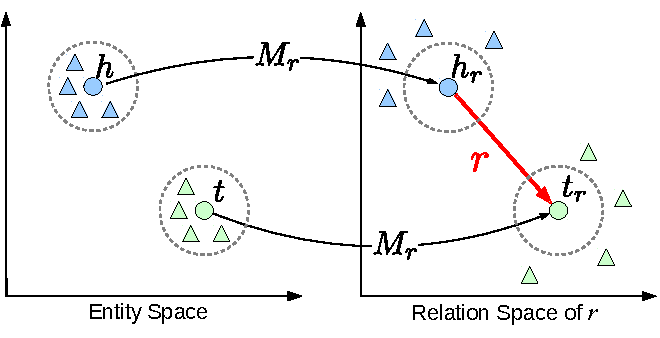
\includegraphics[width=0.8\columnwidth]{figures/trans/model_idea}
  \caption{Simple illustration of TransR.}
  \label{fig:idea}
  \end{figure}

  Knowledge graphs encode structured information of entities and their rich relations. Although a typical knowledge graph may contain millions of entities and billions of relational facts, it is usually far from complete. Knowledge graph completion aims at predicting relations between entities under supervision of the existing knowledge graph. Knowledge graph completion can find new relational facts, which is an important supplement to relation extraction from plain texts.

  Knowledge graph completion is similar to link prediction in social network analysis, but more challenging for the following reasons: (1) nodes in knowledge graphs are entities with different types and attributes; and (2) edges in knowledge graphs are relations of different types. For knowledge graph completion, we not only determine whether there is a relation between two entities or not, but also predict the specific type of the relation.

  For this reason, traditional approach of link prediction is not capable for knowledge graph completion. Recently, a promising approach for the task is embedding a knowledge graph into a continuous vector space while preserving certain information of the graph. Following this approach, many methods have been explored, which will be introduced in detail in Section ``Related Work''.

  Among these methods, TransE \citelatex{bordes2013translating} and TransH \citelatex{wang2014knowledge} are simple and effective, achieving the state-of-the-art prediction performance. TransE, inspired by \citelatex{mikolov2013distributed}, learns vector embeddings for both entities and relationships. These vector embeddings are set in $\mathbb{R}^k$ and we denote  with the same letters in boldface. The basic idea behind TransE is that, the relationship between two entities corresponds to a translation between the embeddings of entities, that is, $\mathbf{h} + \mathbf{r} \approx \mathbf{t}$ when $(h, r, t)$ holds. Since TransE has issues when modeling 1-to-N, N-to-1 and N-to-N relations, TransH is proposed to enable an entity having different representations when involved in various relations.

  Both TransE and TransH assume embeddings of entities and relations being in the same space $\mathbb{R}^k$. However, an entity may have multiple aspects, and various relations focus on different aspects of entities. Hence, it is intuitive that some entities are similar and thus close to each other in the entity space, but are comparably different in some specific aspects and thus far away from each other in the corresponding relation spaces. To address this issue, we propose a new method, which models entities and relations in distinct spaces, i.e., \textbf{entity space} and multiple \textbf{relation spaces} (i.e., relation-specific entity spaces), and performs translation in the corresponding relation space, hence named as TransR.

  The basic idea of TransR is illustrated in Fig. \ref{fig:idea}. For each triple $(h, r, t)$, entities in the entity space are first projected into $r$-relation space as $h_r$ and $t_r$ with operation $M_r$, and then $\mathbf{h}_r + \mathbf{r} \approx \mathbf{t}_r$. The relation-specific projection can make the head/tail entities that actually hold the relation (denoted as colored circles) close with each other, and also get far away from those that do not hold the relation (denoted as colored triangles).

  Moreover, under a specific relation, head-tail entity pairs usually exhibit diverse patterns. It is insufficient to build only a single relation vector to perform all translations from head to tail entities. For example, the head-tail entities of the relation ``location\_location\_contains'' have many patterns such as country-city, country-university, continent-country and so on. Following the idea of piecewise linear regression \citelatex{ritzema1994drainage}, we extend TransR by clustering diverse head-tail entity pairs into groups and learning distinct relation vectors for each group, named as cluster-based TransR (CTransR).

  We evaluate our models with the tasks of link prediction, triple classification and relation fact extraction on benchmark datasets of WordNet and Freebase. Experiment results show significant and consistent improvements compared to state-of-the-art models.


  \section{Related Models}

    \subsection{TransE and TransH}
    As mentioned in Section ``Introduction'', TransE \citelatex{bordes2013translating} wants $\mathbf{h} + \mathbf{r} \approx \mathbf{t}$ when $(h, r, t)$ holds. This indicates that $(\mathbf{t})$ should be the nearest neighbor of $(\mathbf{h} + \mathbf{r})$. Hence, TransE assumes the score function
    \begin{equation}
    f_{r}(h, t) = \|\mathbf{h} + \mathbf{r} - \mathbf{t}\|_{2}^{2}
    \end{equation}
    is low if $(h, r, t)$ holds, and high otherwise.

    TransE applies well to 1-to-1 relations but has issues for N-to-1, 1-to-N and N-to-N relations. Take a 1-to-N relation $r$ for example. $\forall i \in \{0, \ldots, m\}, (h_i, r, t) \in S$. This indicates that $\mathbf{h}_0 = \ldots = \mathbf{h}_m$, which does not comport with the facts.

    To address the issue of TransE when modeling N-to-1, 1-to-N and N-to-N relations, TransH \citelatex{wang2014knowledge} is proposed to enable an entity to have distinct distributed representations when involved in different relations. For a relation $r$, TransH models the relation as a vector $\mathbf{r}$ on a hyperplane with $\mathbf{w}_r$ as the normal vector. For a triple $(h, r, t)$, the entity embeddings $\mathbf{h}$ and $\mathbf{t}$ are first projected to the hyperplane of $\mathbf{w}_r$, denoted as $\mathbf{h}_{\bot}$ and $\mathbf{t}_{\bot}$. Then the score function is defined as
    \begin{equation}
    f_{r}(h, t) = \|\mathbf{h}_{\bot} + \mathbf{r} - \mathbf{t}_{\bot}\|_{2}^{2}.
    \end{equation}
    If we restrict $\|\mathbf{w}_r\|_{2} = 1$, we will have $\mathbf{h}_{\bot} = \mathbf{h} - \mathbf{w}_{r}^{\top}\mathbf{h}\mathbf{w}_{r}$ and $\mathbf{t}_{\bot} = \mathbf{t} - \mathbf{w}_{r}^{\top}\mathbf{t}\mathbf{w}_{r}$. By projecting entity embeddings into relation hyperplanes, it allows entities playing different roles in different relations.

    \subsection{Other Models}
    Besides TransE and TransH, there are also many other methods following the approaches of knowledge graph embedding. Here we introduce several typical models, which will also be compared as baselines with our models in experiments.

    \textbf{Unstructured Model (UM).} UM model \citelatex{bordes2012joint,bordes2014semantic} was proposed as a naive version of TransE by assigning all $\mathbf{r} = \mathbf{0}$, leading to score function $f_r(h, t) =  \|\mathbf{h} - \mathbf{t}\|_{2}^{2}$. This model cannot consider differences of relations.

    \textbf{Structured Embedding (SE).} SE model \citelatex{bordes2011learning} designs two relation-specific matrices for head and tail entities, i.e., $\mathbf{M}_{r, 1}$ and $\mathbf{M}_{r, 2}$, and defines the score function as an $L_1$ distance between two projected vectors, i.e., $f_r(h, t) =  \| \mathbf{M}_{r, 1} \mathbf{h} - \mathbf{M}_{r, 2} \mathbf{t} \|_1$. Since the model has two separate matrices for optimization, it cannot capture precise relations between entities and relations.

    \textbf{Single Layer Model (SLM).} SLM model was proposed as a naive baseline of NTN \citelatex{socher2013reasoning}. The score function of SLM model is defined as
    \begin{equation}
    f_{r}(h, t) = \mathbf{u}_r^\top g (\mathbf{M}_{r, 1} \mathbf{h} + \mathbf{M}_{r, 2} \mathbf{t}),
    \end{equation}
    where $\mathbf{M}_{r, 1}$ and $\mathbf{M}_{r, 2}$ are weight matrices, and $g()$ is the \texttt{tanh} operation. SLM is a special case of NTN when the tensor in NTN is set to $\mathbf{0}$.

    \textbf{Semantic Matching Energy (SME).} SME model \citelatex{bordes2012joint,bordes2014semantic} aims to capture correlations between entities and relations via multiple matrix products and Hadamard product. SME model simply represents each relation using a single vector, which interacts with entity vectors via linear matrix products, with all relations share the same parameters. SME considers two definitions of semantic matching energy functions for optimization, including the linear form
    \begin{equation}
    f_r(h, t) = (\mathbf{M}_{1} \mathbf{h} + \mathbf{M}_{2} \mathbf{r} + \mathbf{b}_1 )^{\top} (\mathbf{M}_{3} \mathbf{t} + \mathbf{M}_{4} \mathbf{r} + \mathbf{b}_2),
    \end{equation}
    and the bilinear form
    \begin{equation}
    f_r(h, t) = \big( (\mathbf{M}_{1} \mathbf{h}) \otimes (\mathbf{M}_{2} \mathbf{r}) + \mathbf{b}_1 \big)^{\top} \big( (\mathbf{M}_{3} \mathbf{t}) \otimes (\mathbf{M}_{4} \mathbf{r}) + \mathbf{b}_2 \big),
    \end{equation}
    where $\mathbf{M}_{1}$, $\mathbf{M}_{2}$, $\mathbf{M}_{3}$ and $\mathbf{M}_{4}$ are weight matrices, $\otimes$ is the Hadamard product, $\mathbf{b}_1$ and $\mathbf{b}_2$ are bias vectors. In \citelatex{bordes2014semantic}, the bilinear form of SME is re-defined with $3$-way tensors instead of matrices.

    \textbf{Latent Factor Model (LFM).} LFM model \citelatex{jenatton2012latent,sutskever2009modelling} considers second-order correlations between entity embeddings using a quadratic form,  and defines a bilinear score function $f_r(h, t) = \mathbf{h}^{\top}\mathbf{M}_r\mathbf{t}$.

    \textbf{Neural Tensor Network (NTN).} NTN model \citelatex{socher2013reasoning} defines an expressive score function for graph embedding as follows,
    \begin{equation}
    f_{r}(h, t) = \mathbf{u}_r^\top g (\mathbf{h}^{\top} \mathbf{M}_r \mathbf{t} + \mathbf{M}_{r, 1} \mathbf{h} + \mathbf{M}_{r, 2}\mathbf{t} + \mathbf{b}_r),
    \end{equation}
    where $\mathbf{u}_r$ is a relation-specific linear layer, $g()$ is the \texttt{tanh} operation, $\mathbf{M}_r \in \mathbb{R}^{d \times d \times k}$ is a $3$-way tensor, and $\mathbf{M}_{r, 1}, \mathbf{M}_{r, 2} \in  \mathbb{R}^{k\times d}$ are weight matrices. Meanwhile, the corresponding high complexity of NTN may prevent it from efficiently applying on large-scale knowledge graphs.

    In experiments we will also compare with \textbf{RESCAL}, a collective matrix factorization model presented in \citelatex{nickel2011three,nickel2012factorizing}.



    \section{Our Method}
    \label{sec:method}

    To address the representation issue of TransE and TransH, we propose TransR, which represent entities and relations in distinct semantic space bridged by relation-specific matrices.

    \subsection{TransR}
    Both TransE and TransH assume embeddings of entities and relations within the same space $\mathbb{R}^k$. But relations and entities are completely different objects, it may be not capable to represent them in a common semantic space. Although TransH extends modeling flexibility by employing relation hyperplanes, it does not perfectly break the restrict of this assumption. To address this issue, we propose a new method, which models entities and relations in distinct spaces, i.e., \textbf{entity space} and \textbf{relation spaces}, and performs translation in relation space, hence named as TransR.

    In TransR, for each triple $(h, r, t)$, entities embeddings are set as $\mathbf{h}, \mathbf{t} \in \mathbb{R}^k$ and relation embedding is set as $\mathbf{r} \in \mathbb{R}^d$. Note that, the dimensions of entity embeddings and relation embeddings are not necessarily identical, i.e., $k \ne d$.

    For each relation $r$, we set a projection matrix $\mathbf{M}_{r} \in \mathbb{R}^{k \times d}$, which may projects entities from entity space to relation space. With the mapping matrix, we define the projected vectors of entities as
    \begin{equation}
    \mathbf{h}_{r} = \mathbf{h}\mathbf{M}_r, \quad \mathbf{t}_{r} = \mathbf{t}\mathbf{M}_r.
    \end{equation}
    The score function is correspondingly defined as
    \begin{equation}
    f_{r}(h, t) = \|\mathbf{h}_r + \mathbf{r} - \mathbf{t}_r\|_{2}^{2}.
    \end{equation}
    In practice, we enforce constraints on the norms of the embeddings $h$, $r$, $t$ and the mapping matrices, i.e. $\forall h, r, t$, we have $\|\mathbf{h}\|_2\le1,\|\mathbf{r}\|_2\le1, \|\mathbf{t}\|_2\le1, \|\mathbf{h}\mathbf{M_r}\|_2\le1, \|\mathbf{t}\mathbf{M_r}\|_2\le1$.

    \subsection{Cluster-based TransR (CTransR)}
    The above mentioned models, including TransE, TransH and TransR, learn a unique vector for each relation, which may be under-representative to fit all entity pairs under this relation, because these relations are usually rather diverse. In order to better model these relations, we incorporate the idea of piecewise linear regression \citelatex{ritzema1994drainage} to extend TransR.

    The basic idea is that, we first segment input instances into several groups. Formally, for a specific relation $r$, all entity pairs $(h, t)$ in the training data are clustered into multiple groups, and entity pairs in each group are expected to exhibit similar $r$ relation. All entity pairs $(h, t)$ are represented with their vector offsets $(\mathbf{h} - \mathbf{t})$ for clustering, where $\mathbf{h}$ and $\mathbf{t}$ are obtained with TransE. Afterwards, we learn a separate relation vector $\mathbf{r}_c$ for each cluster and matrix $\mathbf{M}_{r}$ for each relation, respectively. We define the projected vectors of entities as $\mathbf{h}_{r,c} = \mathbf{h}\mathbf{M}_{r}$ and $\mathbf{t}_{r,c} = \mathbf{t}\mathbf{M}_{r}$, and the score function is defined as
    \begin{equation}
    f_{r}(h, t) = \|\mathbf{h}_{r, c} + \mathbf{r}_c - \mathbf{t}_{r, c}\|_{2}^{2} + \alpha \|\mathbf{r}_{c} - \mathbf{r}\|_{2}^{2},
    \end{equation}
    where $\|\mathbf{r}_{c} - \mathbf{r}\|_{2}^{2}$ aims to ensure cluster-specific relation vector $\mathbf{r}_{c}$ not too far away from the original relation vector $\mathbf{r}$, and $\alpha$ controls the effect of this constraint. Besides, same to TransR, CTransR also enforce constraints on norm of embeddings $h, r, t$ and mapping matrices.

    \subsection{Training Method and Implementation Details}
    We define the following margin-based score function as objective for training
    \begin{equation}
    L = \sum_{(h, r, t) \in S}\sum_{(h', r, t') \in S'}\max \big( 0, f_r(h, t) + \gamma - f_r(h', t')\big),
    \end{equation}
    where $\max(x,y)$ aims to get the maximum between $x$ and $y$, $\gamma$ is the margin, $S$ is the set of correct triples and $S'$ is the set of incorrect triples.

    Existing knowledge graphs only contain correct triples. It is routine to corrupt correct triples $(h, r, t) \in S$ by replacing entities, and construct incorrect triples $(h', r, t') \in S'$. When corrupting the triple, we follow \citelatex{wang2014knowledge} and assign different probabilities for head/tail entity replacement. For those 1-to-N, N-to-1 and N-to-N relations, by giving more chance to replace the ``one'' side, the chance of generating false-negative instances will be reduced. In experiments, we will denote the traditional sampling method as ``unif'' and the new method in \citelatex{wang2014knowledge}  as ``bern''.

    The learning process of TransR and CTransR is carried out using stochastic gradient descent (SGD). To avoid overfitting, we initialize entity and relation embeddings with results of TransE, and initialize relation matrices as identity matrices.


    \section{Experiments and Analysis}
    \label{sec:experiment}

    \subsection{Data Sets and Experiment Setting}
    In this paper, we evaluate our methods with two typical knowledge graphs, built with WordNet \citelatex{miller1995wordnet} and Freebase \citelatex{bollacker2008freebase}. WordNet provides semantic knowledge of words. In WordNet, each entity is a \emph{synset} consisting of several words, corresponding to a distinct \emph{word sense}. Relationships are defined between synsets indicating their lexical relations, such as \texttt{hypernym}, \texttt{hyponym}, \texttt{meronym} and \texttt{holonym}. In this paper, we employ two data sets from WordNet, i.e., \texttt{WN18} used in \citelatex{bordes2014semantic} and \texttt{WN11} used in \citelatex{socher2013reasoning}. \texttt{WN18} contains $18$ relation types and \texttt{WN11} contains $11$. Freebase provides general facts of the world. For example, the triple (Steve Jobs, founded, Apple Inc.) builds a relation of \texttt{founded} between the name entity \emph{Steve Jobs} and the organization entity \emph{Apple Inc}. In this paper, we employ two data sets from Freebase, i.e.,  \texttt{FB15K} used in \citelatex{bordes2014semantic} and \texttt{FB13} used in \citelatex{socher2013reasoning}. We list statistics of these data sets in Table \ref{table:statistics}.

    \begin{table}[h]
    \small
    \centering
    \caption{Statistics of data sets.}
    \label{table:statistics}
    \begin{tabular}{|c|rrrrr|}
    \hline
    Dataset &\#Rel& \#Ent& \#Train& \#Valid& \# Test\\
    \hline
    WN18  & 18     & 40,943  &141,442 & 5,000  & 5,000\\
    FB15K & 1,345 & 14,951 & 483,142 & 50,000& 59,071\\
    WN11  &11       & 38,696 & 112,581 & 2,609  &10,544\\
    FB13   &13       & 75,043 &316,232  &5,908  &23,733\\
    FB40K & 1,336 & 39528 &370,648 &67,946&96,678\\
    \hline
    \end{tabular}
    \end{table}

    \subsection{Link Prediction}
    Link prediction aims to predict the missing $h$ or $t$ for a relation fact triple $(h, r, t)$, used in \citelatex{bordes2011learning,bordes2012joint,bordes2013translating}. In this task, for each position of missing entity, the system is asked to rank a set of candidate entities from the knowledge graph, instead of only giving one best result. As set up in \citelatex{bordes2011learning,bordes2013translating}, we conduct experiments using the data sets WN18 and FB15K.

    In testing phase, for each test triple $(h, r, t)$, we replace the head/tail entity by all entities in the knowledge graph, and rank these entities in descending order of similarity scores calculated by score function $f_r$. Following \citelatex{bordes2013translating}, we use two measures as our evaluation metric: (1) mean rank of correct entities; and (2) proportion of correct entities in top-$10$ ranked entities (Hits@10). A good link predictor should achieve lower mean rank or higher Hits@10. In fact, a corrupted triple may also exist in knowledge graphs, which should be also considered as correct. However, the above evaluation may under-estimate those systems that rank these corrupted but correct triples high. Hence, before ranking we may filter out these corrupted triples which have appeared in knowledge graph. We name the first evaluation setting as ``Raw'' and the latter one as ``Filter''.

    Since we use the same data sets, we compare our models with baselines reported in \citelatex{bordes2013translating,wang2014knowledge}. For experiments of TransR and CTransR, we select learning rate $\lambda$ for SGD among $\{0.1, 0.01, 0.001\}$, the margin $\gamma$ among $\{1, 2, 4\}$ , the dimensions of entity embedding $k$ and relation embedding $d$ among $\{20,50,100\}$ , the batch size $B$ among $\{20, 120, 480, 1440, 4800\}$, and $\alpha$ for CTransR among $\{0.1,0.01,0.001\}$. The best configuration is determined according to the mean rank in validation set.  The optimal configurations are $\lambda = 0.001$, $\gamma= 4$, $k = 50$, $d = 50$, $B = 1440$, $\alpha=0.001$ and taking $L_1$ as dissimilarity on WN18; $\lambda = 0.001$, $\gamma = 1$, $k = 50$, $d = 50$, $B = 4800$, $\alpha=0.01$ and taking $L_1$ as dissimilarity on FB15K. For both datasets, we traverse all the training triplets for $500$ rounds.

    Evaluation results on both WN18 and FB15K are shown in Table \ref{label:link_prediction}. From the table we observe that: (1) TransR and CTransR outperform other baseline methods including TransE and TransH significantly and consistently. It indicates that TransR finds a better trade-off between model complexity and expressivity. (2) CTransR performs better than TransR, which indicates that we should build fine-grained models to handle complicated internal correlations under each relation type. CTransR is a preliminary exploration; it will be our future work to build more sophisticated models for this purpose.  (3) The ``bern'' sampling trick works well for both TransH and TransR, especially on FB15K which have much more relation types.



    \begin{table*}[htb]
    \small
      \centering
      \caption{Evaluation results on link prediction.}
      \label{label:link_prediction}
      \begin{tabular}{|c|rr|rr|rr|rr|}
        \hline
        Data Sets & \multicolumn{4}{|c|}{WN18}&\multicolumn{4}{|c|}{FB15K}\\
        \hline
        
        \multirow{2}{*}{Metric} & \multicolumn{2}{|c|}{Mean Rank} & \multicolumn{2}{|c|}{Hits@10 ($\%$)} & \multicolumn{2}{|c|}{Mean Rank}& \multicolumn{2}{|c|}{Hits@10 ($\%$)} \\
        & Raw &Filter & Raw & Filter & Raw & Filter & Raw & Filter \\
        \hline
        Unstructured \citelatex{bordes2012joint}        &    315  &    304 & 35.3 & 38.2 & 1,074 & 979 &    4.5 &   6.3\\
        RESCAL \citelatex{nickel2011three}               & 1,180  & 1,163 & 37.2 & 52.8 &    828 & 683 &  28.4 & 44.1\\
        SE \citelatex{bordes2011learning}                  & 1,011  &    985 & 68.5 & 80.5 &    273 & 162 &  28.8 & 39.8\\
        SME (linear) \citelatex{bordes2012joint}         &    545  &    533 & 65.1 & 74.1 &    274 & 154 &  30.7 & 40.8\\
        SME (bilinear) \citelatex{bordes2012joint}      &    526  &    509 & 54.7 & 61.3 &    284 & 158 &  31.3 & 41.3\\
        LFM  \citelatex{jenatton2012latent}                 &    469  &   456 & 71.4 & 81.6 &    283 & 164 &  26.0 & 33.1\\
        TransE \citelatex{bordes2013translating}        &    263 &    251 & 75.4 & 89.2 &    243 & 125 &  34.9 & 47.1\\
        TransH (unif) \citelatex{wang2014knowledge} &   318 &    303 & 75.4 & 86.7 &    211 &    84 &  42.5 & 58.5\\
        TransH (bern) \citelatex{wang2014knowledge}&   401 &    388 & 73.0 & 82.3 &    212 &    87 & 45.7 & 64.4\\
         \hline
        TransR (unif)  &232 &219 &           78.3                &91.7&                226&            78 &            43.8 &           65.5\\
        TransR (bern) & 238             &225             &\textbf{79.8}  &92.0 &    \textbf{198}& 77 &  48.2 & 68.7 \\
     CTransR (unif) & 243 & 230& 78.9&\textbf{92.3} & 233&  82  &44&66.3\\
     CTransR (bern) & \textbf{231}            &\textbf{218}             &79.4  &\textbf{92.3} &   199  & \textbf{75} & \textbf{48.4} &\textbf{70.2} \\
        \hline
      \end{tabular}
    \end{table*}

    In Table \ref{label:mapping_property}, we show separate evaluation results by mapping properties of relations \footnote{Mapping properties of relations follows the same rules in \citelatex{bordes2013translating}.} on FB15K. We can see TransR achieves great improvement consistently on all mapping categories of relations, especially when (1) predicting ``1-to-1'' relations, which indicates that TransR provides more precise representation for both entities and relation and their complex correlations, as illustrated in Fig. \ref{fig:idea}; and (2) predicting the \emph{1} side for ``1-to-N'' and ``N-to-1'' relations, which shows the ability of TransR to discriminate relevant from irrelevant entities via relation-specific projection.

    \begin{table*}[htb]
    \small
    \centering
    \caption{Evaluation results on FB15K by mapping properties of relations. ($\%$)}
     \label{label:mapping_property}
    \begin{tabular}{|c|rrrr|rrrr|}
    \hline
    Tasks &\multicolumn{4}{|c|}{Predicting Head(Hits@10)}&\multicolumn{4}{|c|}{Predicting Tail(Hits@10)}\\
    \hline
    Relation Category&1-to-1&1-to-N&N-to-1&N-to-N&1-to-1&1-to-N&N-to-1&N-to-N\\
    \hline
    Unstructured \citelatex{bordes2012joint}           & 34.5  &   2.5 &   6.1 &   6.6 & 34.3 &   4.2 &   1.9 &   6.6\\
    SE \citelatex{bordes2011learning}                     & 35.6  & 62.6 & 17.2 & 37.5 & 34.9 & 14.6 & 68.3 & 41.3\\
    SME (linear)   \citelatex{bordes2012joint}          & 35.1  & 53.7 & 19.0 & 40.3 & 32.7 & 14.9 & 61.6 & 43.3\\
    SME (bilinear) \citelatex{bordes2012joint}         & 30.9  & 69.6 & 19.9 & 38.6 & 28.2 & 13.1 & 76.0 & 41.8\\
    TransE \citelatex{bordes2013translating}          &43.7   & 65.7 & 18.2 & 47.2 & 43.7 & 19.7 & 66.7 & 50.0\\
    TransH (unif)  \citelatex{wang2014knowledge} & 66.7  & 81.7 &  30.2 & 57.4 & 63.7 & 30.1 & 83.2 & 60.8\\
    TransH (bern) \citelatex{wang2014knowledge} & 66.8  & 87.6 &  28.7 & 64.5 & 65.5 & 39.8 & 83.3 & 67.2\\
    \hline
    TransR (unif)  & 76.9&  77.9&\textbf{38.1}&66.9&76.2&38.4&76.2&69.1
    \\
    TransR (bern) & 78.8&\textbf{89.2}&34.1&69.2&79.2&37.4&\textbf{90.4}&72.1
     \\
    CTransR (unif) &78.6&77.8&36.4&68.0&77.4& 37.8& 78.0&70.3\\
    CTransR (bern)& \textbf{81.5}&89.0&34.7&\textbf{71.2}&\textbf{80.8}&38.6&90.1&\textbf{73.8}
    \\
    \hline
    \end{tabular}
    \end{table*}

    \begin{table}[htb]
    \small
    \centering
    \caption{$\langle$Head, Tail$\rangle$ examples of some clusters for the relation ``location\_location\_contains''.}
     \label{label:cluster_example}
    \begin{tabular}{|c|p{0.88\columnwidth}|}
    \hline
    & \multicolumn{1}{|c|}{$\langle$Head, Tail$\rangle$} \\
    \hline
    1 & $\langle$Africa, Congo$\rangle$, $\langle$Asia, Nepal$\rangle$, $\langle$Americas, Aruba$\rangle$,  $\langle$Oceania, Federated States of Micronesia$\rangle$
    \\ \hline
    2 & $\langle$United States of America, Kankakee$\rangle$,
    $\langle$England, Bury St Edmunds$\rangle$,
    $\langle$England, Darlington$\rangle$, $\langle$Italy, Perugia$\rangle$ \\ \hline
    3 & $\langle$Georgia, Chatham County$\rangle$, $\langle$Idaho, Boise$\rangle$, $\langle$Iowa, Polk County$\rangle$, $\langle$Missouri, Jackson County$\rangle$, $\langle$Nebraska, Cass County$\rangle$
    \\ \hline
    4 & $\langle$Sweden, Lund University$\rangle$, $\langle$England, King's College at Cambridge$\rangle$, $\langle$Fresno, California State University at Fresno$\rangle$, $\langle$Italy, Milan Conservatory$\rangle$
    \\\hline
    \end{tabular}
    \end{table}

    Table \ref{label:cluster_example} gives some cluster examples for the relation ``location\_location\_contains'' in FB15K training triples. We can find obvious patterns that: Cluster\#1 is about continent containing country, Cluster\#2 is about country containing city, Cluster\#3 is about state containing county, and Cluster\#4 is about country containing university. It is obvious that by clustering we can learn more precise and fine-grained relation embeddings, which can further help improve the performance of  knowledge graph completion.

    \subsection{Triple Classification}
    Triple classification aims to judge whether a given triple $(h, r, t)$ is correct or not. This is a binary classification task, which has been explored in \citelatex{socher2013reasoning,wang2014knowledge} for evaluation. In this task, we use three data sets, WN11, FB13 and FB15K, following \citelatex{wang2014knowledge}, where the first two datasets are used in \citelatex{socher2013reasoning}.

    We need negative triples for evaluation of binary classification. The data sets WN11 and FB13 released by NTN \citelatex{socher2013reasoning} already have negative triples, which are obtained by corrupting correct triples. As FB15K with negative triples has not been released by previous work, we construct negative triples following the same setting in \citelatex{socher2013reasoning}. For triple classification, we set a relation-specific threshold $\delta_r$. For a triple $(h,r,t)$, if the dissimilarity score obtained by $f_r$ is below $\delta_r$, the triple will be classified as positive, otherwise negative. $\delta_r$ is optimized by maximizing classification accuracies on the validation set.

    For WN11 and FB13, we compare our models with baseline methods reported in \citelatex{wang2014knowledge} who used the same data sets. As mentioned in \citelatex{wang2014knowledge}, for a fair comparison, all reported results are without combination with word embedding.

    Since FB15K is generated by ourselves according to the strategy in \citelatex{socher2013reasoning}, the evaluation results are not able to compare directly with those reported in \citelatex{wang2014knowledge}. Hence, we implement TransE and TransH, and use the NTN code released by \citelatex{socher2013reasoning}, and evaluate on our FB15K data set for comparison.

    For experiments of TransR  we select learning rate $\lambda$ for SGD among $\{0.1, 0.01, 0.001,0.0001\}$, the margin $\gamma$ among $\{1, 2, 4\}$ , the dimensions of entity embedding $k$ , relation embedding $d$ among $\{20,50,100\}$ and the batch size $B$ among $\{20, 120, 480, 960, 4800\}$ . The best configuration is determined according to accuracy in validation set.The optimal configurations are: $\lambda = 0.001$, $\gamma= 4$, $k, d = 20$, $B = 120$  and taking $L_1$ as dissimilarity on WN11; $\lambda = 0.0001$, $\gamma= 2$, $k, d = 100$ and $B = 480$ and taking $L_1$ as dissimilarity on FB13. For both datasets, we traverse all the training triples for $1000$ rounds.

    Evaluation results of triple classification is shown in Table \ref{label:triple_classification}. From Table \ref{label:triple_classification}, we observe that: (1) On WN11, TransR significantly outperforms baseline methods including TransE and TransH. (2) Neither TransE, TransH nor TransR can outperform the most expressive model NTN on FB13. In contrast, on the larger data set FB15K, TransE, TransH and TransR perform much better than NTN. The results may correlate with the characteristics of data sets: There are $1,345$ relation types in FB15K and only $13$ relations types in FB13. Meanwhile, the number of entities and relational facts in the two data sets are close. As discussed in \citelatex{wang2014knowledge}, the knowledge graph in FB13 is much denser than FB15K and even WN11. It seems that the most expressive model NTN can learn complicated correlations using tensor transformation from the dense graph of FB13. In contrast, simpler models are able to better handle the sparse graph of FB15K with good generalization. (3) Moreover, the ``bern'' sampling technique improves the performance of TransE, TransH and TransR on all three data sets.

    As shown in \citelatex{wang2014knowledge}, the training time of TransE and TransH are about $5$ and $30$ minutes, respectively. The computation complexity of TransR is higher than both TransE and TransH, which takes about $3$ hours for training.

    \begin{table}[htb]
    \small
    \centering
    \caption{Evaluation results of triple classification. ($\%$)}
    \label{label:triple_classification}
    \begin{tabular}{|c|r|r|r|r|}
    \hline
    Data Sets & WN11 & FB13 & FB15K \\
    \hline
    SE                   & 53.0 &           75.2  & - \\
    SME (bilinear) & 70.0 &           63.7  & - \\
    SLM                & 69.9 &           85.3  & - \\
    LFM                & 73.8 &           84.3  & - \\
    NTN                & 70.4 &\textbf{87.1} &68.5 \\
    TransE (unif)  & 75.9 &           70.9  & 79.6 \\
    TransE (bern) & 75.9 &           81.5  & 79.2 \\
    TransH (unif)  & 77.7 &           76.5  & 79.0 \\
    TransH (bern) & 78.8 &           83.3  & 80.2 \\ \hline
    TransR (unif)  &85.5  &           74.7  & 81.7 \\
    TransR (bern) &\textbf{85.9}&82.5  & 83.9 \\
    CTransR (bern) & 85.7 & -&\textbf{84.5}\\
    \hline
    \end{tabular}
    \end{table}

    \subsection{Relation Extraction from Text}
    Relation extraction aims to extract relational fact from large-scale plain text, which is an important information source to enrich knowledge graphs. Most exiting methods \citelatex{mintz2009distant,riedel2010modeling,hoffmann2011knowledge,surdeanu2012multi} take knowledge graphs as distant supervision to automatically annotate sentences in large-scale text corpora as training instances, and then extract textual features to build relation classifiers. These methods only use plain texts to reason new relational fact; meanwhile knowledge graph embeddings perform link prediction only based on existing knowledge graphs.

    It is straightforward to take advantage of both plain texts and knowledge graphs to infer new relational facts. In \citelatex{weston2013connecting}, TransE and text-based extraction model were combined to rank candidate facts and achieved promising improvement. Similar improvements are also found over TransH \citelatex{wang2014knowledge}. In this section, we will investigate the performance of TransR when combining with text-based relation extraction model.

    We adopt NYT+FB, also used in \citelatex{weston2013connecting}, to build text-based relation extraction model. In this data set, entities in New York Times Corpus are annotated with Stanford NER and linked to Freebase.

    In our experiments, we implement the same text-based extraction model proposed in \citelatex{weston2013connecting} which is named as Sm2r. For the knowledge graph part, \citelatex{weston2013connecting} used a subset restricted to the top $4$ million entities with $23$ thousand relation types. As TransH has not released the dataset and TransR will take too long to learn from $4$ million entities, we generate a smaller data set FB40K ourselves, which contains all entities in NYT and $1,336$ relation types. For test fairness, from FB40K we remove all triples whose entity pairs have appeared in the testing set of NYT. As compared to previous results in \citelatex{weston2013connecting,wang2014knowledge}, we find that learning with FB40K does not significantly reduce the effectiveness of TransE and TransH. Hence we can safely use FB40K to demonstrate the effectiveness of TransR.

    Following the same method in \citelatex{weston2013connecting}, we combine the scores from text-based relation extraction model with the scores from knowledge graph embeddings to rank test triples, and get precision-recall curves for TransE, TransH and TransR. Since the freebase part of our data set is built by ourselves, different from the ones in \citelatex{wang2014knowledge}, the evaluation results cannot be compared directly with those reported in \citelatex{wang2014knowledge}. Hence, we implement TransE, TransH and TransR by ourselves. We set the embedding dimensions $k, d = 50$, the learning rate $\lambda = 0.001$, the margin $\gamma = 1.0$, $B = 960$, and dissimilarity metric as $L_1$. Evaluation curves are shown in Figure \ref{fig:relation_extraction}.

    \begin{figure}[htb]
    \centering
    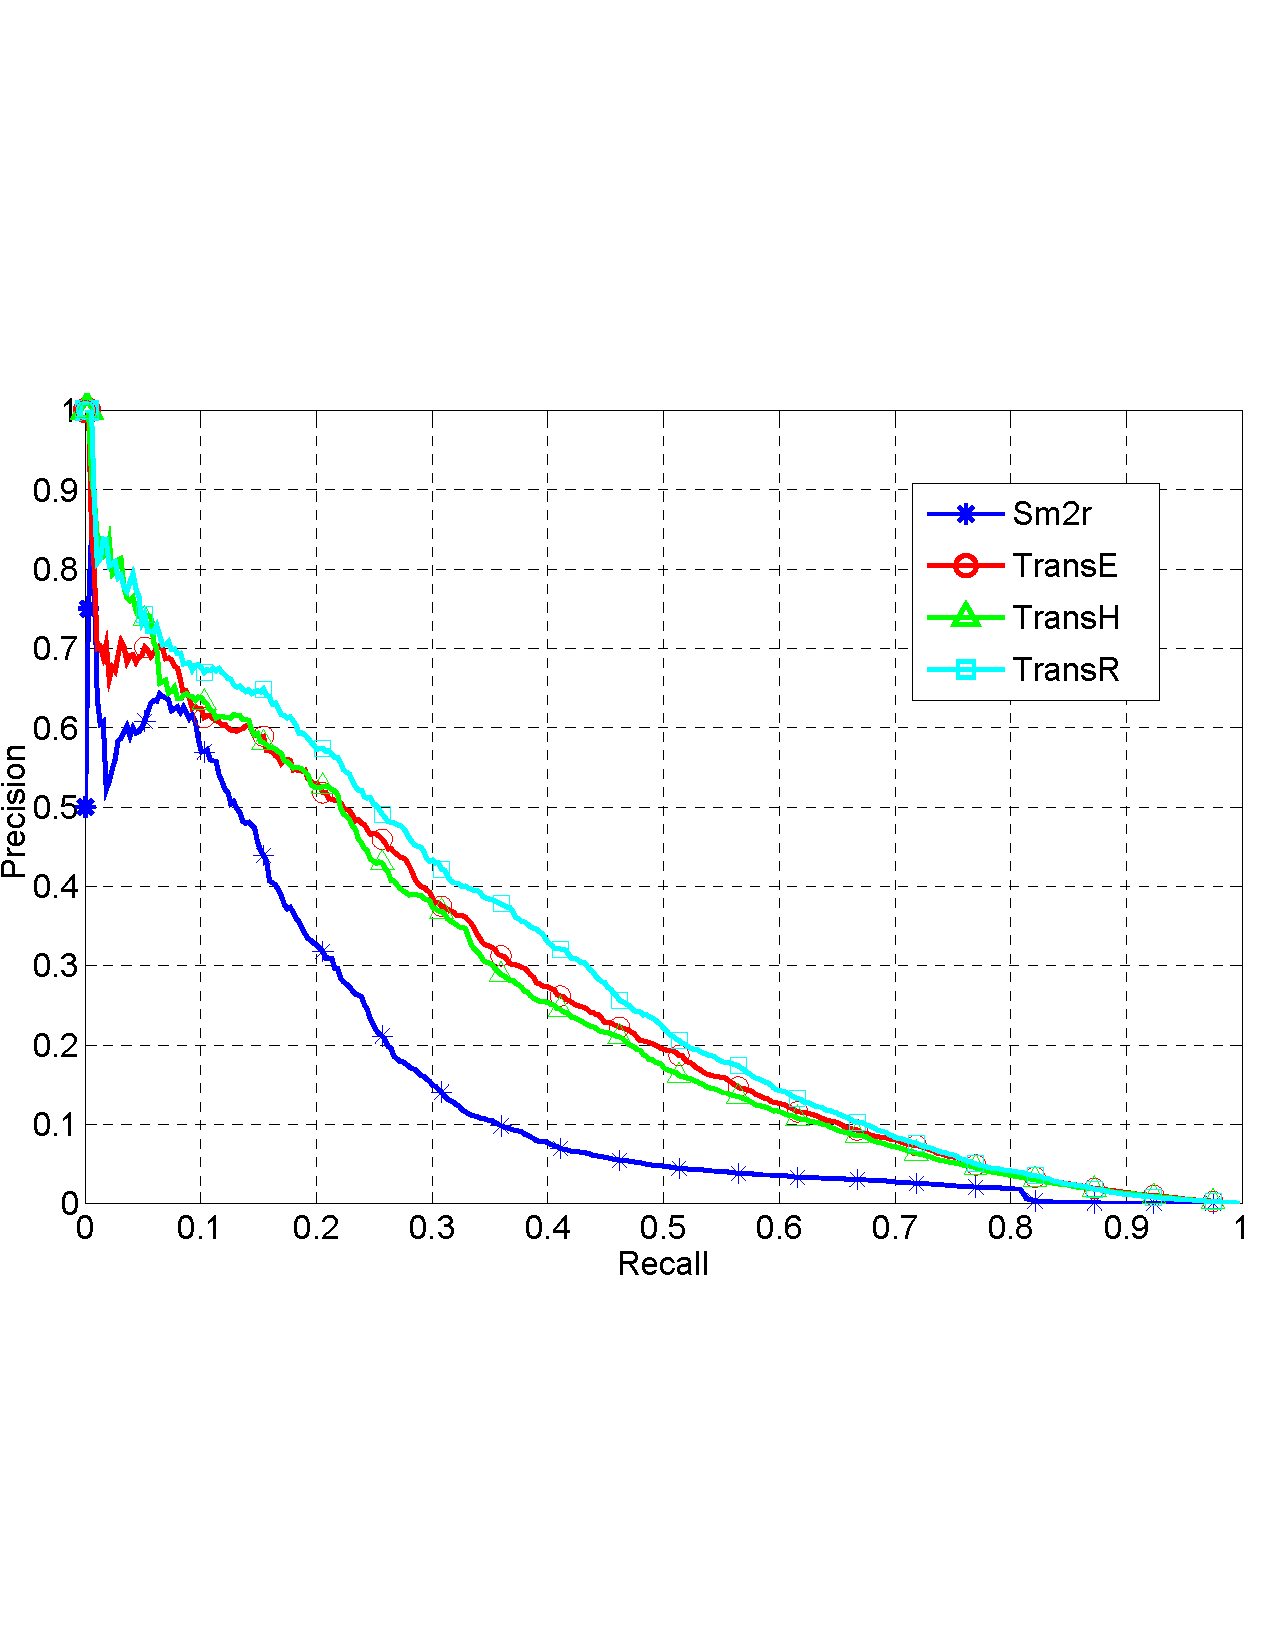
\includegraphics[width=0.8\columnwidth]{figures/trans/RE_text}
    \caption{Precision-recall curves of TransE, TransH and TransR for relation extraction from text.}
    \label{fig:relation_extraction}
    \end{figure}

    From the table we observe that TransR outperforms TransE and is comparable with TransH when recall ranges $[0, 0.05]$, and outperforms all baselines including TransE and TransH when recall ranges $[0.05, 1]$.

    Recently, the idea of embeddings has also been widely used for representing words and texts \citelatex{bengio2003neural,mikolov2013efficient,mikolov2013distributed,mikolov2013linguistic}, which may be used for text-based relation extraction.

    \section{Conclusion}
      In this paper, we propose TransR, a new knowledge graph embedding model. TransR embeds entities and relations in distinct entity space and relation space, and learns embeddings via translation between projected entities. In addition, we also propose CTransR, which aims to model internal complicated correlations within each relation type based on the idea of piecewise linear regression. In experiments, we evaluate our models on three tasks including link prediction, triple classification and fact extraction from text. Experiment results show that TransR achieves consistent and significant improvements compared to TransE and TransH.

\chapter{外文资料的调研阅读报告或书面翻译}

\title{知识图谱填充任务中实体与关系的表示学习}

{\heiti 摘要:} 

知识图谱填充是一个预测知识图谱实体间链接关系类型的任务。在本篇论文中,我们提出了一个知识图谱嵌入的算法来解决这个问题。在最近的研究中,诸如 TransE 和 TransR 这样的模型将关系作为头实体到尾实体之间的转移来对知识图谱进行嵌入。通常,这类算法会将实体和关系在同一个连续空间中进行嵌入。实际上,一个实体可能有多个方面,即在不同关系下拥有不同的意义,这使得在一个统一的空间中建模变的很困难。在本文中,我们提出了叫作 TransR 的模型来将实体和关系在不同空间中嵌入。然后,在这个模型中我们再学习实体空间和关系空间的映射关系,从而将实体从实体空间映射到关系空间中来构建头实体到尾实体之间的转移。在试验中,我们在三个任务上评测了我们的模型,包括链接预测,三元组分类和关系现实抽取。实验结果和之前最好的模型相比有显著的提升,这些模型中包括 TransE 和 TransH。这篇论文的源代码被我们公布在 https://github.com/mrlyk423/relation\_extractio 上。

\section{引言}

  \begin{figure}[htb]
  \centering
  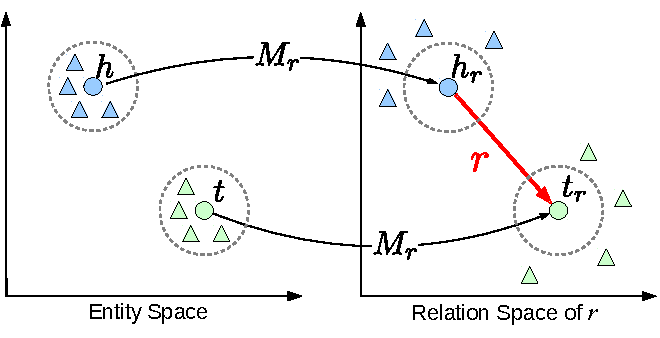
\includegraphics[width=0.8\columnwidth]{figures/trans/model_idea}
  \caption{Simple illustration of TransR.}
  \label{fig_1:idea}
  \end{figure}

知识图谱可以将实体和实体间丰富的关系信息进行结构化。尽管一个经典的知识图谱可能含有数百万个实体和数以亿个关系事实,这个图谱离完善还差的很远。知识图谱填充这个任务就是为了在已有图谱信息的监督下进行学习并能够预测实体间的未知关系。这个任务可以推理出新的关系事实,从而也对从自由文本中进行关系抽取有很重要的作用。

知识图谱填充和社交网络中的链接预测非常相似,但是更具有挑战性,主要原因有以下几点:(1)知识图谱中的节点代表的实体通常具有不同的关系与属性;(2)知识图谱中的边代表的关系也是有不同类型的。对于知识图谱填充,我们不仅需要知道实体之间是否有关系还要知道这个关系是哪种具体的类型。

因为这个原因,传统的用来做链接预测的方法对于图谱填充是不适用的。最近,一个极有发展潜力的模型被提出用来将知识图谱嵌入到一个连续的向量空间中同时在空间中保持图的特性。紧跟着这个工作,大量的方法被尝试和提出,这个我们将会在``相关工作''章节细节阐述。

在这些方法中,TransE \citelatex{bordes2013translating} 和 TransH \citelatex{wang2014knowledge} 最为简洁有效,并且取得了最好的预测效果。受 \citelatex{mikolov2013distributed} 的启发,TransE 将实体和关系都嵌入为空间中的向量。这些向量的维度为 $\mathbb{R}^k$,我们也用加粗的符号来代表对应的向量。Trans 最基本的想法就是将实体之间的关系对应到实体向量间的转移,即知识图谱中的三元组$(h, r, t)$,我们有$\mathbf{h} + \mathbf{r} \approx \mathbf{t}$。因为 TransE 对于 1-to-N、N-to-1、N-to-N 的关系建模有一定的问题,TransH 被提出以便将实体在不同的关系下拥有不同的表示从而适应这种非一对一的关系。

无论是 TransE 还是 TransH 都将实体和关系嵌入到同一个$\mathbb{R}^k$的空间中去。但是,我们之前说到的,一个实体在不同的关系下是有所区别的。因此,有这样一个显而易见的现象,相似的实体会在空间上非常接近,但是在不同的关系背景下我们又希望它们有区分性,即距离上要相互远离,这两者在同一个空间中是矛盾的。为了解决这个问题,我们提出了一个新的方法,将实体和关系在各自的空间中进行嵌入,例如实体在一个实体空间中,不同类型的关系在不同的关系空间中,并且要构建一个映射机制能够将实体从实体空间映射到不同的关系空间中去,我们将这个方法命名为 TransR。

TransR 的基础想法如图\ref{fig_1:idea}所示。对于一个给定的三元组$(h, r, t)$,实体首先从实体空间被映射到关系$r$所在的关系空间中去成为$h_r$和$t_r$,映射为$M_r$,然后有$\mathbf{h}_r + \mathbf{r} \approx \mathbf{t}_r$。通过这样的一种映射,我们可以使得头尾实体能够在空间中具有相似性,而在不同的关系中又有不同的空间表现。

更进一步,即使在同一个类型的关系下,实体间的潜在关联也是具有多样性的。所以即使对于每一个关系都构建一个向量也是不够的。举个例子,头尾之间的关系``行政区划覆盖''可能具有很多中关系模式,比如``国家-城市''、``国家-大学''、``洲-国家''等等。受到分段线性回归 \citelatex{ritzema1994drainage} 的启发,我们通过将头尾实体间的潜在关系进行聚类,并为每一个聚类的簇单独建立向量表示的方法进一步拓展了TransR,并且命名为 CTransR。
 
我们在三个任务上评测了我们的模型,包括链接预测,三元组分类和关系现实抽取,数据也是从WordNet和Freebase中抽取出专门用来做性能评测的标准数据集。实验结果和之前最好的模型相比有显著的提升,体现了我们模型的有效性。

\section{相关工作}

    \subsection{TransE和TransH}

    正如我们在``引言''中介绍的那样,TransE \citelatex{bordes2013translating} 希望图谱中的三元组$(h, r, t)$满足$\mathbf{h} + \mathbf{r} \approx \mathbf{t}$。这表明$(\mathbf{t})$在空间中应该是最接近$(\mathbf{h} + \mathbf{r})$的。因此,TransE 定义了这样一个评分函数:
    \begin{equation}
    f_{r}(h, t) = \|\mathbf{h} + \mathbf{r} - \mathbf{t}\|_{2}^{2},
    \end{equation}
    函数值越低代表$(h, r, t)$存在的可能性越大,反之亦然。

    TransE 在 1-to-1 的关系上表现突出,但是在 N-to-1, 1-to-N 以及 N-to-N 这些类别的关系上存在问题。我们以一个 1-to-N 类别的关系$r$作为案例。$\forall i \in \{0, \ldots, m\}, (h_i, r, t) \in S$. 这表明$\mathbf{h}_0 = \ldots = \mathbf{h}_m$,然而这和实际现象是违背的。

    为了解决TransE在 N-to-1, 1-to-N 以及 N-to-N 类别关系上的问题,TransH \citelatex{wang2014knowledge} 被提了出来,并用以将实体在不同关系的环境下嵌入不同的分布式表示向量里去。对于任意的关系$r$,TransH 将关系建模为一个法向量为$\mathbf{w}_r$的超平面上的向量$\mathbf{r}$。对于任意一个三元组$(h, r, t)$,



    实体的向量$\mathbf{h}$和$\mathbf{t}$首先被映射到$\mathbf{w}_r$的超平面上成为$\mathbf{h}_{\bot}$和$\mathbf{t}_{\bot}$,接着和TransE类似的定义出评分函数:
    \begin{equation}
    f_{r}(h, t) = \|\mathbf{h}_{\bot} + \mathbf{r} - \mathbf{t}_{\bot}\|_{2}^{2}。
    \end{equation}
    在$\|\mathbf{w}_r\|_{2} = 1$的约束下, 参数满足$\mathbf{h}_{\bot} = \mathbf{h} - \mathbf{w}_{r}^{\top}\mathbf{h}\mathbf{w}_{r}$,以及$\mathbf{t}_{\bot} = \mathbf{t} - \mathbf{w}_{r}^{\top}\mathbf{t}\mathbf{w}_{r}$。正是通过将实体向量映射到关系超平面上,我们使得实体在不同的关系环境下有不同的表示。


    \subsection{其他模型}
    除了 TransE 和 TransH,还有许多其他模型可以用来对知识图谱进行嵌入。这里我们介绍一些经典的模型方案,并且也会作为我们的实验对比在实验环节体现。

    \textbf{Unstructured Model (UM)。} UM \citelatex{bordes2012joint,bordes2014semantic} 是一个简化版本的 TransE,即在 TransE 的基础上满足$\mathbf{r} = \mathbf{0}$, 此时我们的评分函数为$f_r(h, t) =  \|\mathbf{h} - \mathbf{t}\|_{2}^{2}$。很显然,这个模型无法处理实体间多种关系的情况。

    \textbf{Structured Embedding (SE)。} SE \citelatex{bordes2011learning} 为头实体和尾实体设计了不同的变换矩阵,比如$\mathbf{M}_{r, 1}$和$\mathbf{M}_{r, 2}$,并且在这些变换矩阵的基础上定义了$L_1$距离的评分函数,$f_r(h, t) =  \| \mathbf{M}_{r, 1} \mathbf{h} - \mathbf{M}_{r, 2} \mathbf{t} \|_1$。由于模型具有两个独立的变换矩阵,因此不能捕获实体和关系之间的精确关系。

    \textbf{Single Layer Model (SLM)。} SLM 是 NTN \citelatex{socher2013reasoning}的简化版本。评分函数如下:
    \begin{equation}
    f_{r}(h, t) = \mathbf{u}_r^\top g (\mathbf{M}_{r, 1} \mathbf{h} + \mathbf{M}_{r, 2} \mathbf{t}),
    \end{equation}
    这里$\mathbf{M}_{r, 1}$和$\mathbf{M}_{r, 2}$是权重矩阵,$g()$是\texttt{tanh}操作。SLM 是 NTN 在张量被设置为$\mathbf{0}$时的特例。


    \textbf{Semantic Matching Energy (SME)。} SME \citelatex{bordes2012joint,bordes2014semantic} 可以通过多重矩阵乘法和哈达玛积来获取实体和关系之间的相关性。SME 模型将关系表示为一个独立的向量,这些向量通过线性矩阵乘积与实体向量相互作用,并且关系向量内部共享相同的参数。SME 定义了两个语义能量函数用于优化,包括线性形式:
    \begin{equation}
    f_r(h, t) = (\mathbf{M}_{1} \mathbf{h} + \mathbf{M}_{2} \mathbf{r} + \mathbf{b}_1 )^{\top} (\mathbf{M}_{3} \mathbf{t} + \mathbf{M}_{4} \mathbf{r} + \mathbf{b}_2),
    \end{equation}
    和双线性形式:
    \begin{equation}
    f_r(h, t) = \big( (\mathbf{M}_{1} \mathbf{h}) \otimes (\mathbf{M}_{2} \mathbf{r}) + \mathbf{b}_1 \big)^{\top} \big( (\mathbf{M}_{3} \mathbf{t}) \otimes (\mathbf{M}_{4} \mathbf{r}) + \mathbf{b}_2 \big),
    \end{equation}
    这里$\mathbf{M}_{1}$,$\mathbf{M}_{2}$,$\mathbf{M}_{3}$和$\mathbf{M}_{4}$是权重矩阵,$\otimes$是哈达玛积,$\mathbf{b}_1$和$\mathbf{b}_2$是线性偏置向量。在 \citelatex{bordes2014semantic}的工作中,SME 的双线性形式被重新定义为三路张量而不是矩阵。

    \textbf{Latent Factor Model (LFM)。} LFM \citelatex{jenatton2012latent,sutskever2009modelling} 考虑使用实体嵌入之间的二阶相关性来定义一个双线性评分函数$f_r(h, t) = \mathbf{h}^{\top}\mathbf{M}_r\mathbf{t}$。

    \textbf{Neural Tensor Network (NTN)。} NTN \citelatex{socher2013reasoning} 定义了一个表达能力很强的评分函数:
    \begin{equation}
    f_{r}(h, t) = \mathbf{u}_r^\top g (\mathbf{h}^{\top} \mathbf{M}_r \mathbf{t} + \mathbf{M}_{r, 1} \mathbf{h} + \mathbf{M}_{r, 2}\mathbf{t} + \mathbf{b}_r),
    \end{equation}
    这里$\mathbf{u}_r$是一个针对关系的线性变换层,$g()$是\texttt{tanh}操作,$\mathbf{M}_r \in \mathbb{R}^{d \times d \times k}$是一个三路的张量,$\mathbf{M}_{r, 1}, \mathbf{M}_{r, 2} \in  \mathbb{R}^{k\times d}$则是权重矩阵。在表达能力强的同时,NTN 的高复杂度使得它很难在大规模知识图谱上被应用。

    考虑到时间问题,在实验部分我们将会和\textbf{RESCAL}, 一个 \citelatex{nickel2011three,nickel2012factorizing} 提出的类似的矩阵分解算法来对比。


    \section{我们的模型}
    \label{sec:method}

    为了解决 TransE 和 TransH 在表示学习中的一些问题,我们提出了 TransR ,该模型可以将实体和关系在不同的空间中进行嵌入,并且通过特殊的矩阵将实体映射到关系空间中。

    \subsection{TransR}


    TransE 和 TransH 都将实体和关系嵌入到相同的维度为$\mathbb{R}^k$的空间中去。实际上,关系和实体是完全不同概念的事物,在同一个语义空间中将这些东西同时嵌入是有一些问题的。尽管 TransH 通过关系的超平面假设让实体在不同关系下具有了一定的自由度,但是仍然无法突破同一个空间带来的约束。为解决这个问题,我们提出了新的方法将实体和关系嵌入到不同的空间中去,比如\textbf{实体空间}和\textbf{关系空间},并且在关系空间中采取了类似 TransE 和 TransH 的转移特性,我们将模型命名为TransR。

    在 TransR 中,对于每一个三元组$(h, r, t)$,实体向量定义为$\mathbf{h}, \mathbf{t} \in \mathbb{R}^k$,关系向量定义为$\mathbf{r} \in \mathbb{R}^d$。值得注意的是,因为在不同空间中,所以实体和关系向量的维度可以是不同的,即$k \ne d$。

    对于特定的关系$r$,我们定义映射矩阵$\mathbf{M}_{r} \in \mathbb{R}^{k \times d}$将实体映射到关系空间中。通过这个映射矩阵,我们可以定义映射之后的实体向量:
    \begin{equation}
    \mathbf{h}_{r} = \mathbf{h}\mathbf{M}_r, \quad \mathbf{t}_{r} = \mathbf{t}\mathbf{M}_r。
    \end{equation}
    因而,评分函数可以定义为:
    \begin{equation}
    f_{r}(h, t) = \|\mathbf{h}_r + \mathbf{r} - \mathbf{t}_r\|_{2}^{2}。
    \end{equation}
    在此基础上,我们加上了约束使得$h$, $r$, $t$的向量和映射矩阵满足$\forall h, r, t$,$\|\mathbf{h}\|_2\le1,\|\mathbf{r}\|_2\le1, \|\mathbf{t}\|_2\le1, \|\mathbf{h}\mathbf{M_r}\|_2\le1, \|\mathbf{t}\mathbf{M_r}\|_2\le1$.

    \subsection{基于聚类的 TransR (CTransR)}
    之前提到的模型,包括 TransE, TransH 和 TransR,均是为每个关系学习一个单独的向量,但是这往往是不能覆盖所有实体对之间的潜在关系的,因为这些关系往往在不同的语境下具有多样性。为了更好的将一种关系下的多个子类型区分开来,我们引入了多重线性回归 \citelatex{ritzema1994drainage} 的思路来拓展 TransR。

    基本的思路是这样的,我们首先我们将训练的案例分为若干组。对于特定的关系$r$,所有训练数据中蕴含这个关系的实体对$(h, t)$将会被聚类到若干组中,并且聚类到同一组里的实体对拥有相同的关系并且和$r$的向量接近。对于所有的实体对$(h, t)$ 将使用它们的向量运算$(\mathbf{h} - \mathbf{t})$来聚类。然后为每个聚类结果学习得到一个单独的新的向量$\mathbf{r}_c$和映射矩阵$\mathbf{M}_{r}$。我们将映射的实体向量定义为$\mathbf{h}_{r,c} = \mathbf{h}\mathbf{M}_{r}$和$\mathbf{t}_{r,c} = \mathbf{t}\mathbf{M}_{r}$,而评分函数也被定义为:
    \begin{equation}
    f_{r}(h, t) = \|\mathbf{h}_{r, c} + \mathbf{r}_c - \mathbf{t}_{r, c}\|_{2}^{2} + \alpha \|\mathbf{r}_{c} - \mathbf{r}\|_{2}^{2},
    \end{equation}
    这里$\|\mathbf{r}_{c} - \mathbf{r}\|_{2}^{2}$用来约束聚类成的关系向量$\mathbf{r}_{c}$离原始的关系向量$\mathbf{r}$在距离上不是很远,$\alpha$用来调节这个约束对损失函数的影响。除此以外,和 TransR 一样,CTransR 也要强行约束$h, r, t$的向量以及映射矩阵。

    \subsection{训练方法和实现细节}
    我们定义了以下一个基于边界值的损失函数作为我们的训练目标,
    \begin{equation}
    L = \sum_{(h, r, t) \in S}\sum_{(h', r, t') \in S'}\max \big( 0, f_r(h, t) + \gamma - f_r(h', t')\big),
    \end{equation}
    这里$\max(x,y)$用来在$x$ 和 $y$中选取一个最大值,$\gamma$ 就是边界值, $S$是正例的三元组集合而$S'$是负例的三元组集合。

    知识图谱中只存在正例三元组,所以我们通过从正例三元组集合$(h, r, t) \in S$中替换实体来构建负例三元组集合$(h', r, t') \in S'$。当替换三元组的实体时,我们遵循 \citelatex{wang2014knowledge} 中提出的方法并且采用不同概率来替换头尾实体。对于 1-to-N、N-to-1、N-to-N 这样的关系, 我们会对其中``1''这边的实体给予更多的关注和更大的概率来生成负例。在试验中,我们将过去一贯的采样方法命名为``unif''并且将这个 \citelatex{wang2014knowledge} 提出的新的方法命名为``bern''。

    TransR 和 CTransR 的模型学习方法采用了随机梯度下降(stochastic gradient descent,SGD)。为了避免过拟合,我们用 TransE 的结果来初始化实体和关系向量,并且用单位阵来初始化映射矩阵。


    \section{实验和分析}
    \label{sec:experiment}

    \subsection{数据集合和实验设置}
    在这篇论文中,我们在两个经典数据集合上评测了我们的方法,WordNet \citelatex{miller1995wordnet} 和 Freebase \citelatex{bollacker2008freebase}。WordNet 提供了一个词语级别的语义知识图谱。在 WordNet 中,每个实体都是一个包含若干个词语的\emph{同义词集合}并对应一个单独的\emph{词语意义}。而关系则被定义为同义词集合之间的词汇关联,比如\texttt{上位词}, \texttt{下位词}, \texttt{局部词} and \texttt{整体词}。在本文中,我们采用了两个来源于 WordNet 的数据集合,其中\texttt{WN18}曾被用在 \citelatex{bordes2014semantic} 中,而\texttt{WN11}被用在 \citelatex{socher2013reasoning} 中。\texttt{WN18}包含了$18$种关系类型,而\texttt{WN11}包含了$11$中关系类型。Freebase 中提供的是这个世界上的通用知识。举个例子,三元组(乔布斯, 建立, 苹果公司)表述了在姓名实体\emph{乔布斯}和组织实体\emph{苹果公司}之间的关系为\texttt{建立}关系,即乔布斯建立了苹果公司。在本篇论文中,我们同样采用了两个来源于 Freebase 的数据集合,\texttt{FB15K} 曾被用在 \citelatex{bordes2014semantic} 中,而 \texttt{FB13} 曾被用在 \citelatex{socher2013reasoning} 中。我们将数据集合的具体数据罗列在表\ref{table_1:statistics}中。

    \begin{table}[h]
    \small
    \centering
    \caption{Statistics of data sets.}
    \label{table_1:statistics}
    \begin{tabular}{|c|rrrrr|}
    \hline
    Dataset &\#Rel& \#Ent& \#Train& \#Valid& \# Test\\
    \hline
    WN18  & 18     & 40,943  &141,442 & 5,000  & 5,000\\
    FB15K & 1,345 & 14,951 & 483,142 & 50,000& 59,071\\
    WN11  &11       & 38,696 & 112,581 & 2,609  &10,544\\
    FB13   &13       & 75,043 &316,232  &5,908  &23,733\\
    FB40K & 1,336 & 39528 &370,648 &67,946&96,678\\
    \hline
    \end{tabular}
    \end{table}

    \subsection{链接预测}
    链接预测是用来预测三元组$(h, r, t)$中缺失实体$h$或$t$的任务,并且在 \citelatex{bordes2011learning,bordes2012joint,bordes2013translating} 这些工作中被使用过。在本任务中,对于每一个缺失的实体,模型将被要求用所有的知识图谱里的实体作为候选项并进行排名,而不是单纯给出一个最优的预测结果。和之前 \citelatex{bordes2011learning,bordes2013translating} 的工作一样,我们在 WN18 和 FB15K 上进行了实验。

    在测试阶段,对于每个被测试到的三元组$(h, r, t)$,我们用知识图谱中的其他实体作为候选项来替换头实体或者尾实体,并且以降序顺序给出这些实体的评分函数$f_r$。和 \citelatex{bordes2013translating} 一样,我们使用了两种评测方式:(1) 正确的实体评分函数的平均排名(Mean Rank);(2) 正确的实体排名在前$10$的比例,即十命中率(Hits@10)。一个优秀的链接预测模型应当获得较低的平均排名和较高的十命中率。实际上,一个被人为构建的负例三元组有可能是存在于知识图谱中的,实际上这不应当被视作负例。然而,上述的评测方法可能低估了这些三元组对评测结果的影响。因此,在对候选排名之前我们先将这些三元组过滤掉,然后再用上述的评测。我们将原来的评测称为``Raw''而将之后过滤之后的评测称为``Filter''。

    因为采用了相同的数据集合,我们对比了我们的模型和之前论文报告的结果,这些论文包括 \citelatex{bordes2013translating,wang2014knowledge}。对于 TransR 和 CTransR 的实验,我们从$\{0.1, 0.01, 0.001\}$之中为 SGD 的学习率$\lambda$;从$\{1, 2, 4\}$选择边界值$\gamma$;从$\{20,50,100\}$中选择实体和关系的维度$k$和$d$;从$\{20, 120, 480, 1440, 4800\}$中选择一批次训练的数据规模$B$。对于 CTransR,我们从$\{0.1,0.01,0.001\}$中选择约束参数$\alpha$。我们通过验证集的平均排名来决定最好的参数。
    对于 WN18,我们采用了$L_1$距离,最优的参数为$\lambda = 0.001$,$\gamma= 4$,$k = 50$,$d = 50$,$B = 1440$,$\alpha=0.001$。对于 FB15K,我们采用了$L_1$距离,最优的参数为$\lambda = 0.001$,$\gamma = 1$,$k = 50$,$d = 50$,$B = 4800$,$\alpha=0.01$。对于这两个数据集合,我们均训练$500$轮。

    WN18 和 FB15K 上的评测结果被罗列在表\ref{label_1:link_prediction}中。从表中我们可以看出:


     (1) TransR 和 CTransR 比其他模型包括 TransE 和 TransH 要表现突出很多。这表明 TransR 在效率和复杂程度上找到了一个更好的权衡。(2) CTransR 比 TransR 要表现优异,这表明我们应当构建更细粒度的模型来解决同一个关系下复杂的多样性和相关性。CTransR 只是一个初步的尝试,之后我们会在工作中尝试使用更精细的模型来解决这个问题。(3) ``bern''采样的效果在 TransH 和 TransR上都比之前的采样有提升, 尤其是在拥有更多关系的 FB15K 上。

    \begin{table*}[htb]
    \small
      \centering
      \caption{链接预测的评测结果。}
      \label{label_1:link_prediction}
      \begin{tabular}{|c|rr|rr|rr|rr|}
        \hline
        Data Sets & \multicolumn{4}{|c|}{WN18}&\multicolumn{4}{|c|}{FB15K}\\
        \hline
        
        \multirow{2}{*}{Metric} & \multicolumn{2}{|c|}{Mean Rank} & \multicolumn{2}{|c|}{Hits@10 ($\%$)} & \multicolumn{2}{|c|}{Mean Rank}& \multicolumn{2}{|c|}{Hits@10 ($\%$)} \\
        & Raw &Filter & Raw & Filter & Raw & Filter & Raw & Filter \\
        \hline
        Unstructured \citelatex{bordes2012joint}        &    315  &    304 & 35.3 & 38.2 & 1,074 & 979 &    4.5 &   6.3\\
        RESCAL \citelatex{nickel2011three}               & 1,180  & 1,163 & 37.2 & 52.8 &    828 & 683 &  28.4 & 44.1\\
        SE \citelatex{bordes2011learning}                  & 1,011  &    985 & 68.5 & 80.5 &    273 & 162 &  28.8 & 39.8\\
        SME (linear) \citelatex{bordes2012joint}         &    545  &    533 & 65.1 & 74.1 &    274 & 154 &  30.7 & 40.8\\
        SME (bilinear) \citelatex{bordes2012joint}      &    526  &    509 & 54.7 & 61.3 &    284 & 158 &  31.3 & 41.3\\
        LFM  \citelatex{jenatton2012latent}                 &    469  &   456 & 71.4 & 81.6 &    283 & 164 &  26.0 & 33.1\\
        TransE \citelatex{bordes2013translating}        &    263 &    251 & 75.4 & 89.2 &    243 & 125 &  34.9 & 47.1\\
        TransH (unif) \citelatex{wang2014knowledge} &   318 &    303 & 75.4 & 86.7 &    211 &    84 &  42.5 & 58.5\\
        TransH (bern) \citelatex{wang2014knowledge}&   401 &    388 & 73.0 & 82.3 &    212 &    87 & 45.7 & 64.4\\
         \hline
        TransR (unif)  &232 &219 &           78.3                &91.7&                226&            78 &            43.8 &           65.5\\
        TransR (bern) & 238             &225             &\textbf{79.8}  &92.0 &    \textbf{198}& 77 &  48.2 & 68.7 \\
     CTransR (unif) & 243 & 230& 78.9&\textbf{92.3} & 233&  82  &44&66.3\\
     CTransR (bern) & \textbf{231}            &\textbf{218}             &79.4  &\textbf{92.3} &   199  & \textbf{75} & \textbf{48.4} &\textbf{70.2} \\
        \hline
      \end{tabular}
    \end{table*}

    在表\ref{label_1:mapping_property}中,我们将关系分类并且分别表现了实验结果。\footnote{关系的映射方法我们遵循 \citelatex{bordes2013translating} 中的规则。} 在FB15K上,我们可以发现 TransR 在所有分类后的关系上都获得了最好的结果,尤其是 (1) 预测 ``1-to-1'' 关系时,TransR为实体和关系及其复杂的相关性提供了更精确的表示。正如图\ref{fig_1:idea}所示的那样;(2) 预测 ``1-to-N'' 和 ``N-to-1'' 关系时,TransR通过关系特定投影来区分相关实体的能力得到了体现。

    \begin{table*}[htb]
    \small
    \centering
    \caption{将关系分类后在 FB15K 上的评测结果。($\%$)}
     \label{label_1:mapping_property}
    \begin{tabular}{|c|rrrr|rrrr|}
    \hline
    Tasks &\multicolumn{4}{|c|}{Predicting Head(Hits@10)}&\multicolumn{4}{|c|}{Predicting Tail(Hits@10)}\\
    \hline
    Relation Category&1-to-1&1-to-N&N-to-1&N-to-N&1-to-1&1-to-N&N-to-1&N-to-N\\
    \hline
    Unstructured \citelatex{bordes2012joint}           & 34.5  &   2.5 &   6.1 &   6.6 & 34.3 &   4.2 &   1.9 &   6.6\\
    SE \citelatex{bordes2011learning}                     & 35.6  & 62.6 & 17.2 & 37.5 & 34.9 & 14.6 & 68.3 & 41.3\\
    SME (linear)   \citelatex{bordes2012joint}          & 35.1  & 53.7 & 19.0 & 40.3 & 32.7 & 14.9 & 61.6 & 43.3\\
    SME (bilinear) \citelatex{bordes2012joint}         & 30.9  & 69.6 & 19.9 & 38.6 & 28.2 & 13.1 & 76.0 & 41.8\\
    TransE \citelatex{bordes2013translating}          &43.7   & 65.7 & 18.2 & 47.2 & 43.7 & 19.7 & 66.7 & 50.0\\
    TransH (unif)  \citelatex{wang2014knowledge} & 66.7  & 81.7 &  30.2 & 57.4 & 63.7 & 30.1 & 83.2 & 60.8\\
    TransH (bern) \citelatex{wang2014knowledge} & 66.8  & 87.6 &  28.7 & 64.5 & 65.5 & 39.8 & 83.3 & 67.2\\
    \hline
    TransR (unif)  & 76.9&  77.9&\textbf{38.1}&66.9&76.2&38.4&76.2&69.1
    \\
    TransR (bern) & 78.8&\textbf{89.2}&34.1&69.2&79.2&37.4&\textbf{90.4}&72.1
     \\
    CTransR (unif) &78.6&77.8&36.4&68.0&77.4& 37.8& 78.0&70.3\\
    CTransR (bern)& \textbf{81.5}&89.0&34.7&\textbf{71.2}&\textbf{80.8}&38.6&90.1&\textbf{73.8}
    \\
    \hline
    \end{tabular}
    \end{table*}

    \begin{table}[htb]
    \small
    \centering
    \caption{$\langle$头实体, 尾实体$\rangle$对于``location\_location\_contains''关系聚类的样例。}
     \label{label_1:cluster_example}
    \begin{tabular}{|c|p{0.88\columnwidth}|}
    \hline
    & \multicolumn{1}{|c|}{$\langle$头实体, 尾实体$\rangle$} \\
    \hline
    1 & $\langle$Africa, Congo$\rangle$, $\langle$Asia, Nepal$\rangle$, $\langle$Americas, Aruba$\rangle$,  $\langle$Oceania, Federated States of Micronesia$\rangle$
    \\ \hline
    2 & $\langle$United States of America, Kankakee$\rangle$,
    $\langle$England, Bury St Edmunds$\rangle$,
    $\langle$England, Darlington$\rangle$, $\langle$Italy, Perugia$\rangle$ \\ \hline
    3 & $\langle$Georgia, Chatham County$\rangle$, $\langle$Idaho, Boise$\rangle$, $\langle$Iowa, Polk County$\rangle$, $\langle$Missouri, Jackson County$\rangle$, $\langle$Nebraska, Cass County$\rangle$
    \\ \hline
    4 & $\langle$Sweden, Lund University$\rangle$, $\langle$England, King's College at Cambridge$\rangle$, $\langle$Fresno, California State University at Fresno$\rangle$, $\langle$Italy, Milan Conservatory$\rangle$
    \\\hline
    \end{tabular}
    \end{table}

    表\ref{label_1:cluster_example} 给出 FB15K 中``location\_location\_contains''关系的一些聚类示例。我们可以发现:聚类\#1是关于大陆包含国家, 聚类\#2是国家包含城市,聚类\#3是区域包含乡村, 聚类\#4是国家包含大学。很明显,通过聚类,我们可以学习更精确和细粒度的关系嵌入,有助于进一步提高知识图谱的填充性能。


    \subsection{三元组分类}
    三元组分类是一个判断给定三元组$(h, r, t)$正确与否的任务。这是一个二分类任务,已经在 \citelatex{socher2013reasoning,wang2014knowledge} 等工作中作为评测方式。在这个任务上我们采用了 WN11,FB13 和 FB15K 来进行测试,并且和 \citelatex{wang2014knowledge}的设置保持一致。

    我们需要负例三元组来进行二分类测试。在 NTN \citelatex{socher2013reasoning} 中,数据集合 WN11 和 FB13 已经有了负面的三元组。但对于 FB15K 来说却没有之前工作公开发布的负例三元组,我们采用了 \citelatex{socher2013reasoning} 中使用到的负例生成算法设定。对于三元组分类,我们设置了一个特殊的阈值$\delta_r$。对于三元组$(h,r,t)$,如果评分函数的结果低于$\delta_r$,那么三元组将会被认为是正确的,反之则是错误的。$\delta_r$ 通过最大化验证集上的分类精度来进行优化。


    对于 WN11 和 FB13, 我们比较了我们的模型以及 \citelatex{wang2014knowledge} 中汇报的结果在相同的参数设定下。如 \citelatex{wang2014knowledge} 中提到的,为了公平比较,所有报告的结果都不与字嵌入进行组合。

    由于 FB15K 是根据 \citelatex{socher2013reasoning} 中的策略自行生成的,因此评估结果无法直接与 \citelatex{wang2014knowledge} 中报告的结果进行比较。因此,我们实现 TransE 和 TransH,并使用 \citelatex{socher2013reasoning} 发布的NTN代码,并对我们的FB15K数据集进行评估进行比较。

    对于 TransR 的实验来说,我们从$\{0.1, 0.01, 0.001, 0.0001\}$之中为 SGD 的学习率$\lambda$;从$\{1, 2, 4\}$选择边界值$\gamma$;从$\{20,50,100\}$中选择实体和关系的维度$k$和$d$;从$\{20, 120, 480, 1440, 4800\}$中选择一批次训练的数据规模$B$。我们通过验证集的平均排名来决定最好的参数。
    对于 WN11,我们采用了$L_1$距离,最优的参数为$\lambda = 0.001$,$\gamma= 4$,$k = 20$,$d = 20$,$B = 120$,$\alpha=0.001$。对于 FB13,我们采用了$L_1$距离,最优的参数为$\lambda = 0.0001$,$\gamma = 2$,$k = 100$,$d = 100$,$B = 480$,$\alpha=0.01$。对于这两个数据集合,我们均训练$1000$轮。

    三元组分类的评估结果如表\ref{label_1:triple_classification}所示。从表\ref{label_1:triple_classification},我们观察到:(1) 在WN11上,TransR 显著优于包括 TransE 和 TransH 在内的方法。(2) TransE,TransH 和 TransR 都不能超过 FB13 上最具表现力的型号NTN。相比之下,在较大的数据集 FB15K 上,TransE,TransH 和 TransR 的性能要好于NTN。结果可能与数据集的特征有关:FB15K 中有 $1,345$种关系类型,而 FB13 中只有$13$关系类型。同时,两个数据集中的实体数量和关系事实相近。如 \citelatex{wang2014knowledge} 中讨论到的,FB13 中的知识图谱比 FB15K 甚至 WN11 更稠密。某种程度上最具表现力的模型 NTN 可以从 FB13 的密集图中使用张量变换来学习复杂的相关性。相比之下,更简单的模型能够更好地处理 FB15K 这样的稀疏图,并具有良好的泛化能力。(3) 此外,``Bern''采样技术提高了 TransE,TransH 和 TransR 在所有三个数据集上的性能。

    如 \citelatex{wang2014knowledge} 所示,TransE 和 TransH 的训练时间分别为$5$分钟和$30$分钟。TransR 的计算复杂度高于 TransE 和 TransH,训练耗时大约为$3$小时。

    \begin{table}[htb]
    \small
    \centering
    \caption{三元组分类的评测结果。 ($\%$)}
    \label{label_1:triple_classification}
    \begin{tabular}{|c|r|r|r|r|}
    \hline
    Data Sets & WN11 & FB13 & FB15K \\
    \hline
    SE                   & 53.0 &           75.2  & - \\
    SME (bilinear) & 70.0 &           63.7  & - \\
    SLM                & 69.9 &           85.3  & - \\
    LFM                & 73.8 &           84.3  & - \\
    NTN                & 70.4 &\textbf{87.1} &68.5 \\
    TransE (unif)  & 75.9 &           70.9  & 79.6 \\
    TransE (bern) & 75.9 &           81.5  & 79.2 \\
    TransH (unif)  & 77.7 &           76.5  & 79.0 \\
    TransH (bern) & 78.8 &           83.3  & 80.2 \\ \hline
    TransR (unif)  &85.5  &           74.7  & 81.7 \\
    TransR (bern) &\textbf{85.9}&82.5  & 83.9 \\
    CTransR (bern) & 85.7 & -&\textbf{84.5}\\
    \hline
    \end{tabular}
    \end{table}

    \subsection{文本中的关系抽取}

    关系提取旨在从大规模纯文本中提取关系事实,这是丰富知识图谱的重要信息来源。当前大量的方法 \citelatex{mintz2009distant,riedel2010modeling,hoffmann2011knowledge,surdeanu2012multi}将大量文本语料库中的句子通过知识图谱作为距离监督来自动注释形成训练数据,然后提取文本特征来构建关系分类器。这些方法只使用纯文本来推断新的关系事实,与此同时,知识图谱嵌入则是仅基于现有的知识图谱进行链接预测。


    所以,利用纯文本和知识图谱来推断新的关系事实是很直接的想法。在 \citelatex{weston2013connecting} 中,模型将 TransE 和基于文本的提取模型相结合,对候选事实进行排序,取得了有效的效果提升。TransH \citelatex{wang2014knowledge} 也发现了类似的效果改进。在本节中,我们将结合基于文本的关系提取模型来研究 TransR 的性能。

    我们使用了 NYT+FB 数据集合,这个数据集合也被用在 \citelatex{weston2013connecting} 的工作中来构建基于文本的关系提取模型。在这个数据集中,纽约时代周刊文本内容(New York Times Corpus)中的实体用 Stanford NER 来注释并链接到 Freebase 中的实体上。

    在我们的实验中,我们实现了 \citelatex{weston2013connecting} 提出的基于文本的提取模型,并且命名为Sm2r。对于知识图谱部分,\citelatex{weston2013connecting} 使用了上限最高$4$百万个实体的子集,同时有$23000$个关系类型。由于 TransH 尚未发布数据集,且 TransR 将需要花费很长时间才能从$4$百万个实体的数据中学习到嵌入,我们自己生成了一个较小的数据集 FB40K,其中包含 NYT 中的所有实体和$1336$个关系类型。为了测试公平,从 FB40K 我们删除实体对出现在 NYT 测试集中的所有三元组。 与以前的结果 \citelatex{weston2013connecting,wang2014knowledge} 相比,我们发现使用 FB40K 进行学习并不会显着降低 TransE 和 TransH 的有效性。因此,我们可以安全地使用 FB40K 来证明 TransR 的有效性。

    按照在\citelatex{weston2013connecting}中相同的方法,我们将基于文本的关系提取模型的分数与知识图谱嵌入的分数相结合来进行排序,并获得 TransE,TransH 和 TransR 的准确率召回率曲线。由于我们的数据集的 Freebase 部分是由我们自己构建的,与 \citelatex{wang2014knowledge} 不同,评估结果不能直接与 \citelatex{wang2014knowledge} 中报告的结果进行比较。因此,我们自己实施 TransE,TransH 和 TransR。我们将嵌入维度 $k, d = 50$,学习率$\lambda = 0.001$,边界距离$\gamma = 1.0$,$B = 960$,并且采用了$L_1$距离。评估曲线如图\ref{fig_1:relation_extraction}所示。

    \begin{figure}[htb]
    \centering
    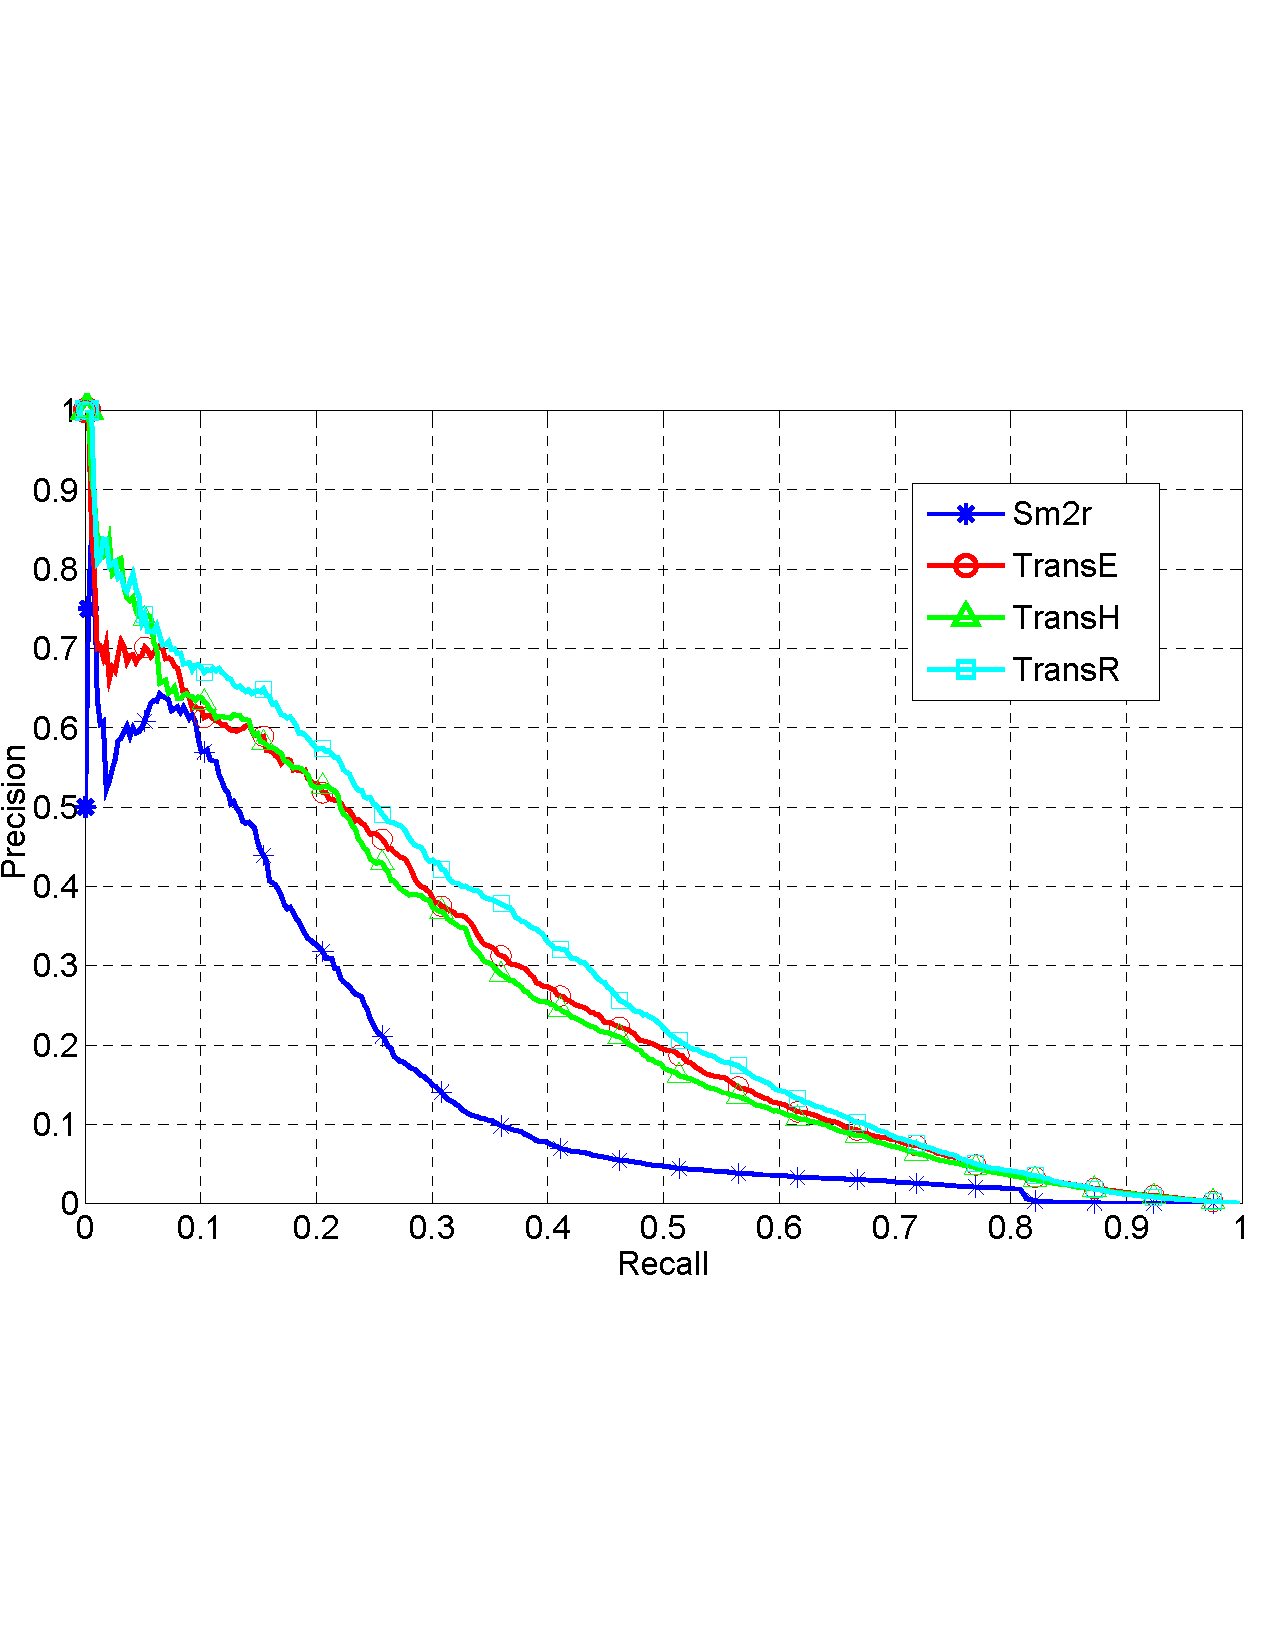
\includegraphics[width=0.8\columnwidth]{figures/trans/RE_text}
    \caption{TransE, TransH 和 TransR 在关系抽取任务上的准确召回率曲线。}
    \label{fig_1:relation_extraction}
    \end{figure}

    从表中我们观察到,当召回范围为$[0,0.05]$时,TransR 优于 TransE,与 TransH 相当,并且当召回范围为$[0.05,1]$时,则超越所有的模型,包括 TransE 和 TransH。

    最近嵌入的想法也被广泛地用于表示单词和文本的工作中 \citelatex{bengio2003neural,mikolov2013efficient,mikolov2013distributed,mikolov2013linguistic},这些都可以在未来用于基于文本的关系提取任务中。

    \section{结论}
    在本文中,我们提出了一种新的知识图谱嵌入模型 TransR。TransR 将实体和关系嵌入不同的实体空间和关系空间中,并通过投影实体转换到关系空间来进行学习嵌入。此外,我们还提出了 CTransR,其目的是基于分段线性回归的思想来模拟每个关系类型内部的复杂的相关性。在实验中,我们对三个任务进行评估,包括链接预测,三元组分类和文本中的关系提取。实验结果表明,与 TransE 和 TransH 相比,TransR 获得了相当一致和显著的效果改进。


% \begin{translationbib}
\bibliographystylelatex{plain}
\bibliographylatex{ref/refs1}
% \end{translationbib}













% \chapter{其它附录}
% 前面两个附录主要是给本科生做例子。其它附录的内容可以放到这里,当然如果你愿意,可
% 以把这部分也放到独立的文件中,然后将其 \cs{input} 到主文件中。
